\chapter{General Mathematical Framework for Runtime Reconfigurable NoC Synthesis}
\label{cha:ch6}
  \begin{figure}%[htb]
  \centering
  % Requires \usepackage{graphicx}
 % \epsfig{file=t_calc.eps}
  \includegraphics[width=1\columnwidth]{overall_22.eps}
  \vskip -1mm
  \caption{\textbf{Overview of the proposed mathematical framework. The reconfigurable NoC system and its associated applications  are characterized through the proposed system and application graphical models. Then the optimization to the network structural configuration is performed by exploiting the submodular property of the problem. In case of a valid solution does not exist, we introduce the relaxation on problem constraints to obtain a feasible solution while preserve the optimality bound.  } }
  \label{fig:concept}
  \vskip -7mm
\end{figure}

\noindent Workloads induced by real world applications demonstrate strong spatio-temporal variability. Heterogeneous application tasks create inter-coupled traffic patterns with time-varying data and control dependencies exacerbating the workloads requirements running over a large scale NoC-based manycore platform~\cite{bogdan2015mathematical}. For instance, big-data applications like biological simulations~\cite{xue2014disease} usually exhibit high dimensionality in their task structures~\cite{xue_NOCS2014_paper}, which are also varying vastly as a function of widely ranged objectives and unpredictable user input. Consequently, the failure to capture such variations through the development of a best-fit NoC-based system, translates to systems that are prone to computation, communication and power inefficiencies.

\indent To address the spatio-temporal behavior of applications, prior research efforts have focussed on two design methodologies, namely the offline analysis of applications and optimization of application specific NoC architectures and the development of on-line optimization techniques. For instance, application-specific NoC synthesis has been well studied to achieve best-possible performance given a specific application. The synthesis usually generates well optimized NoC configurations and application mappings that are superior to baseline design in terms of energy efficiency and performance \cite{singh2013accelerating}\cite{srinivasan2006linear}, application-specific performance (NoC-based accelerators)\cite{majumder2013high}, reliability \cite{zou2013reliability}, lifetime cost \cite{meyer2010cost}. Such optimization considers one or a subset of applications and captures their traffic pattern and task structures. The synthesis is static with no adaptivity and performed prior to its practical deployment, assuming the application structure is not changing over time. Thus performance is very well optimized if only a fixed set of  applications are considered throughout the life cycle of the platform and the applications are almost temporally homogenous. However, the assumptions made before the synthesis usually do not hold. In reality, it is rarely the case that a dedicated NoC is solely developed for exclusive tasks processing. Instead, the NoC is usually used as fundamental communication infrastructure that integrates a set of heterogeneous processing entities that are expected to run a wide range of applications upon deployment. Most of  applications are very diverse in terms of communication patterns and, more importantly, the traffic patterns are also changing over time. Thus, the statically customized network structure could hardly be a feasible traffic carrier that brings good performance in general cases. 

As an alternative to application specific NoC, the reconfigurable NoCs address this problem by changing their structural features \cite{chen2013smart}\cite{jackson2010skip}, routing algorithm \cite{qian2015fsnoc}, resource management strategy \cite{lee2013adaptive}\cite{kobbe2011distrm}, task assignments \cite{singh2013mapping} to fit to time-varying application requirements. In spite of their successful application in diverse settings, we still lack of a solid theoretical foundation upon which an analytical design methodology could be built to optimize the reconfiguration with optimality guarantees in general cases. Most previous reconfigurable NoCs are proposed, evaluated and validated through a subset of experimental instances without looking at entire problem space from a mathematical perspective. 
%In what follows, we will first formally set up the reconfigurable NoC platform and introduce an array of definitions that help to enrich the model expressivity. Then, as a case study, we will formulate the NoC runtime reconfiguration as optimization problem considering the case where application is characterized through a time-dependent graphical model(e.g., time-varying application task graph or dataflow graph). We will show this optimization problem is NP-hard and prove its \textit{submodularity}. By exploring the submodular property, we propose a greedy heuristics with bounded optimality. 
To address the above-mentioned problems, we propose \textit{a general mathematical modeling framework considering the spatio-temporal characteristics of workloads} and make the following novel contributions:
\begin{itemize}
\item We propose a \textbf{mathematical framework} for capturing the \textbf{dynamic nature} of reconfigurable NoC and applications that enables the formulation of major reconfigurable NoC optimization problems. Our analytical formalism can be applied to arbitrary network topologies and sizes, routing, or heterogeneous resource allocation problems.
\item We illustrate the efficacy of this formalism by formulating the \textbf{NoC reconfiguration as a dynamic optimization problem}. We prove that this optimization is NP-hard and demonstrate that our mathematical formulation satisfies the \textbf{submodularity property} justifying that our proposed greedy based algorithms can attain the optimality region.
\item We evaluate the impact of the proposed mathematical formalism by solving the NoC reconfiguration problem. The experimental results show a $52.3\%$ reduction in network latency, increased capability of handling heavy traffic and $30.2\%$ in energy reduction for our lightweight reconfigurable NoC when compared to baseline design.
\end{itemize}

The paper is organized as follows: In Section II, we formally set up the reconfigurable NoC platform and introduce several definitions that help to enrich the model expressivity. Section III presents a case study of the NoC runtime reconfiguration problem considering the case where application is characterized through a time-dependent graphical model (e.g., time-varying application graph). We show this optimization problem is NP-hard and prove its \textit{submodularity}. By exploiting the submodularity property, we propose greedy heuristics with bounded optimality. Sections IV and V summarize our experimental results and our main achievements.

\section{Mathematical Modeling and Optimization Framework}
\subsection{Architectural Modeling Framework}
\noindent \textbf{Definition 1:}\label{def:noc} \textit{A \textbf{reconfigurable network-on-chip} (NoC) is defined as a \textbf{connected dynamic directed graph} $G(t)=(N(t),E(t);\gamma(t),\mathcal C)$ at time $t$, where $n_{i} \in N(t)$ is a tile and represents a collection of functional units, and $E(t)$ denotes the collection of physical links between different nodes in $N(t)$. The $e_{i,j} \in E(t)$ denotes the link from $n_{i}$ to $n_{j}$.}

We should note that $N(t)$ is the set of enabled network functional units (e.g.,  DSPs, general processors, customized processing elements, memories or communication transceivers). The composition of $N(t)$ can change as the subset of nodes are enabled or disabled over time. Also, the reconfigurable NoC usually takes advantage of different switching techniques for best possible performance under diverse workloads.  Therefore, $e_{i,j}$ could be a regular link between two routers or a direct link established between tiles without interfacing with routers. To distinguish between regular and circuit links, we introduce the following definition:

\noindent \textbf{Definition 2:}{ \textit{Edge $e_{i,j}$ is a \textbf{circuit link} if there exists a direct link from $n_{i}$ to $n_{j}$ that allows circuit switching. $E(t)$ induces a function $\mathcal I: E(t) \rightarrow R$ such that $e_{i,j}$ is a circuit link if and only if $\mathcal I(e_{i,j})=1$}.}\label{def:circuit}

The circuit switching link is set up in the regular network to improve throughput over critical traffic path in reconfigurable NoCs.  Circuit switching reserves the entire bandwidth of the dedicated link and skips all routing stages, thus improving greatly the communication throughput when used between a pair of nodes. By connecting different circuit links together, it is possible for a subset of nodes to communicate over such dedicated circuit links for faster data exchange. To characterize such collection of nodes, we introduce the circuit component concept as follows:

\noindent \textbf{Definition 3:}{ \textit{A subset $N'(t) \subseteq N(t)$ is a \textbf{circuit component} $\mathcal T$ if and only if for any pair of nodes $ n_i$ and $n_j \in N'(t)$, there exists a circuit link between them.}\label{def:circuit_component}

A circuit component $\mathcal T$ in $G(t)$ forms a connected subgraph enabling data transfer over dedicated links with augmented bandwidth and reduced latency. For example, %a trivial circuit component is just a single node and 
the simplest circuit component is a pair of nodes with a direct link that skips the routers at both ends. Generally speaking, the reconfiguration of NoC can be viewed as a process of enabling circuit components in the regular network to provide express ways for critical data transmission. 

\noindent \textbf{Definition 4:}{ The \textit{$\gamma(t): N(t) \times N(t) \rightarrow G(t)$ is the \textbf{routing function} at time $t$ that maps a pair of nodes $n_{i}$ and $n_{j}$ to a subgraph $G'(t)$ of $G(t)$ such that: i) $n_{i},n_{j} \in G'(t)$ and ii) there exists at least a path from $n_i$ to $n_j$. } 

\noindent Of note, the $(N(t),E(t);\gamma(t))$ forms a 3-tuple that defines a regular NoC without reconfiguration  features, where $N(t)$ and $E(t)$ characterize its structural properties. $\gamma(t)$ denotes all possible paths for data exchange. 
\begin{figure}%[htb]
  \centering
  % Requires \usepackage{graphicx}
 % \epsfig{file=t_calc.eps}
  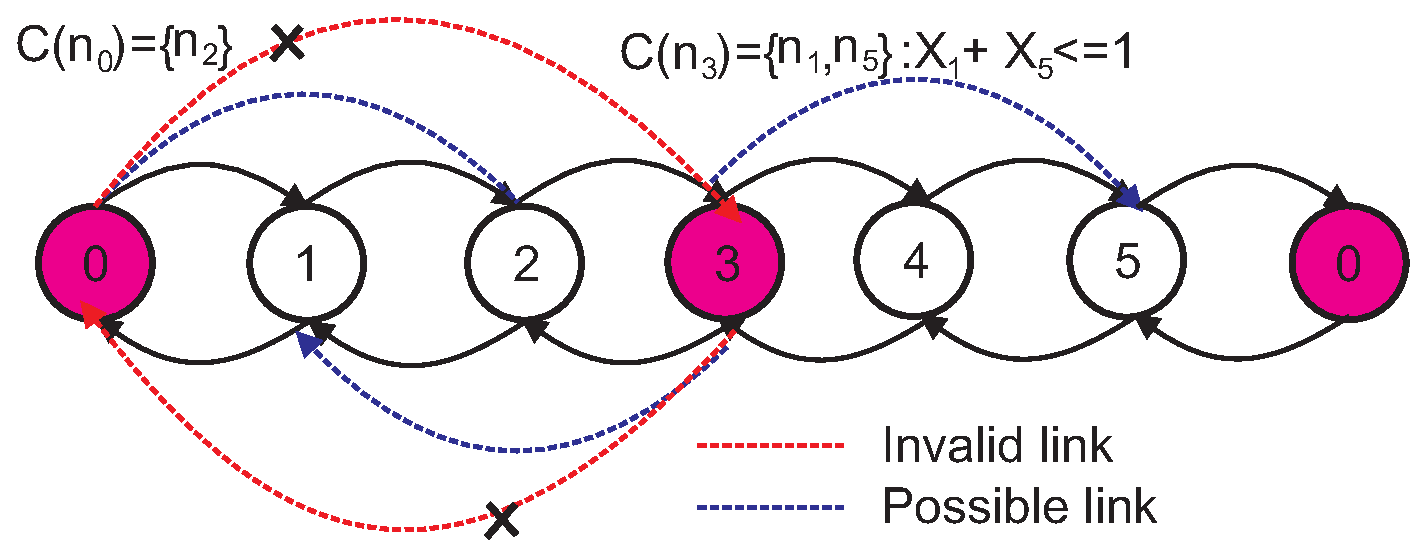
\includegraphics[width=0.8\columnwidth]{alter_set.eps}
  \vskip -1mm
  \caption{\textbf{Augmented connectivity sets are shown for $n_{0}$ and $n_{3}$. $n_{3}$ is configurable to set up link with $n_1$ and $n_5$ whereas both links can not be established at the same time. Similar link to $n_0$ is invalid due to physical limitation.} }
  \label{fig:augment}
  \vskip -6mm
\end{figure}

To be able to model and express the reconfiguration capability, we define the \textit{augmented connectivity function} $\mathcal C$:

\noindent \textbf{Definition 5:} \textit{ $\mathcal C: N(t)\rightarrow 2^{N(t)} $ is the \textbf{augmented connectivity function} (ACF) that associates each node $n_{i} \in E(t)$ at time $t$ with a subset of nodes $\mathcal C(n_{i})=\{n_{j}|n_{j} \in N(t)\}$, to which $e_{i,j}$ could be possibly set up. The set $\mathcal C(n_{i})$ is called \textbf{augmented connectivity set} (ACS).}

By definition, $\mathcal C(n_{i})$ denotes all the possible links that could be alternatively established for $n_{i}$ other than the current links in $\{e_{i,j}|e_{i,j} \in E(t)\}$. We should note that the detailed form of $\mathcal C$ and its range are limited by the physical constraints in a specific architecture. For instance in Figure \ref{fig:augment}, a physical link can not be inserted between $n_3$ and $n_0$ that are too far away from each other given physical limitations (e.g., propagation delay should be less than one cycle). Moreover, a link might not be set up from $n_i$ to $n_{j}$ even if $n_{j} \in \mathcal C(n_i)$. Such constraint comes mostly from architectural limitations which forbid some links from being set up simultaneously  as shown in Figure \ref{fig:augment}. To consider such cases, we introduce a set of constraints associated with $\mathcal C(n_i)$. Let $X_{j}$ be a binary variable such that $X_{j}=1$ if $n_{j} \in \mathcal C(n_i)$ and $e_{i,j}$ is set up. Otherwise, $X_{j}=0$.
\begin{equation}\label{eq:C_constr}
\Sigma \alpha_{j}X_{j}\leq K 
\end{equation}
where, $\alpha_{j} \in \{0,1\}$ represents whether $X_{j}$ is masked or not in the constraints. $K \in \mathcal N$ denotes the maximum number of links that can be established simultaneously. Equation~\eqref{eq:C_constr} defines a constraint, which encodes the physical limitation that a subset of nodes in $\mathcal C(n_i)$ can not connect to $n_i$ at the same time. By changing the configuration of $\{\alpha_{j}\}$, eq.~\eqref{eq:C_constr} forms an array of constraints that capture all such physical limitations.  Thus, we can define the reconfigurable NoC in the general case:

\noindent \textbf{Definition 6 (reconfigurability):} \textit{A node $n_{i}$ is reconfigurable if and only if $C(n_i) \neq \emptyset$. An NoC system $G(t)=(N(t),E(t);\gamma(t),\mathcal C)$ is reconfigurable at time $t$ if there exists at least one node $n_i \in N(t) $ that is reconfigurable.}

\noindent Definition 6 formally defines the reconfigurability. An NoC system $G(t)$ is reconfigurable as long as any one of its nodes has non-empty ACS. By picking up nodes from ACS and constructing new edges over time, $E(t)$ evolves as a function of reconfiguration decisions made prior to time $t$. Of note, Definition 1 enforces the connectivity of a given NoC system. Therefore, the routing algorithm $\gamma(t)$ will also change accordingly to guarantee all the nodes are reachable. Combined with the dynamics of $N(t)$, $G(t)=(N(t),E(t);\gamma(t),\mathcal C)$ describes a dynamical system with time-varying structural characteristics, i.e., $N(t)$, $E(t)$ and $\gamma(t)$, driven by the reconfiguration decisions made upon $\mathcal C(n_i)$ over time. By introducing attributes of interest and associating them with $G(t)$ and application tasks, we are able to construct the theoretical basis on which general NoC reconfiguration could be formulated as optimization problems. To provide an illustrative example of this framework, we present the runtime NoC reconfiguration optimization problem given time-dependent workloads characterized by graphical models.
\subsection{Application Modeling Framework}
Generally speaking, any runtime NoC reconfiguration is an optimization process that searches for the best-fit network structural configurations and application task assignments (i.e, mapping of tasks to specific tiles), given an objective function and a set of constraints. In contrast to application-specific NoC synthesis, runtime optimization is an online process repeatedly synchronized with the time-dependent characteristics of the running applications. This process usually consists of two phases: an execution phase and an optimization phase. In the optimization phase, the optimization will take the profile of applications as input and decide on a best possible network configuration for the execution phase. Profiling the application is a very complex research topic and several models were developed in different contexts. A detailed discussion is beyond the scope of this work. Next, we consider profiling applications via graphical models although the proposed NoC system model $G(t)$ has no constraints on profiling techniques.

\noindent \textbf{Definition 7:}\label{def:app} \textit{ An application $\mathcal A(t)$ is a \textbf{dynamical directed graph} $\mathcal A(t)=(V(t),C(t);\mathcal P(\Sigma,\mathcal F))$ at time $t$. Each vertex $v_{i} \in V(t)$ is a task of the application. $c_{i,j} \in C(t)$ represents a directed data/control dependency from task $v_i$ to task $v_{j}$. }
 
Each application $\mathcal A(t)$ induces a profiling system $\mathcal P(\Sigma,\mathcal F)$. $\Sigma$ is the finite functionality alphabet given specific application context. It contains symbols that characterize the functionality of interest. Functionality profiling function $\mathcal F:V \rightarrow 2^{\Sigma}$ relates each task $v_{i}$ of $\mathcal A(t)$ at time $t$ with a finite set of symbols defined in $\Sigma$ as functionality requirement set $\mathcal F(v_{i})$. To provide some intuition, $\Sigma$ can be as simple as an integer set $\{0,1,2,3\}$ in context of numeric computation where $2$ and $3$ represent ``addition" and ``multiplication". $0$ and $1$ represent ``integer" and ``floating-point", respectively. $\mathcal F$ will induce a functionality requirement set for each node $v_i$. A node $v_i$ with $\mathcal F(v_i)=\{1,2,3\}$ requires floating-point addition and multiplication operations, while a node $v_j$ with $\mathcal F(v_j)=\{0,2\}$ requires only integer addition. By changing alphabet $\Sigma$ based on application context, i.e., application task profiled with interested details, $\mathcal P(\Sigma,\mathcal F)$ is able to characterize each task with sufficiently many mathematical details.

Moreover, we will use the same profiling system $\mathcal P(\Sigma,\mathcal F)$ to characterize the ``capabilities" of each tile $n_{i} \in G(t)$ such that we can easily compare capabilities of the NoC $G(t)$ with the functionality requirements from the application domain. This constitutes the foundation for application task assignment. For each $n_{i}$ of $G(t)$, we define $\mathcal F(n_i)$ as capability set such that, an application task $v_{i}$ with functionality requirement set $\mathcal F(v_i)$ can be mapped to $n_i$ \textit{only if} $\mathcal F(v_i) \subseteq \mathcal F(n_i)$. 
 
Each directed edge $c_{i,j} \in C(t)$ is characterized by a data generation process $P_{c_{i,j}}(k,t)=P\{\mathcal N(t)=k,k \in N\}$ where $\mathcal N(t)$ is a counting process which denotes the number of packets generated in time interval $[t,t+\tau]$. $P_{c_{i,j}}(k,t)$ captures the time-varying behavior of the application. To provide some intuition, the data generation process could be a Poisson process if no memory-effect is present or it could be a fractal process governed by power-laws exhibiting long-range memory \ dependency. Therefore, for an execution phase of length $T$, the \textit{average traffic volume} $q(c_{i,j})$ from task $v_i$ to task $v_j$ could be calculated as follows,
\begin{equation}\label{eq:traffic_vol}
q(c_{i,j})=\int_{t}^{t+T} \int_{-\infty}^{\infty} kP_{c_{i,j}}(k,t) dk dt
\end{equation}

We define by $b(c_{i,j})$ the minimal bandwidth requirement for communication from $v_{i}$ to $v_{j}$. It should be noted that this requirement comes from the execution time constraints posed by the associated tasks. We define $\mathcal B(e_{i,j}, \mathcal I(e_{i,j}))$ as the bandwidth provided by the link $e_{i,j} \in E(t)$ given NoC system $G(t)$. Attribute $\mathcal I(e_{i,j})$ is introduced in $\mathcal B$ to consider the bandwidth difference between regular and circuit links. We check the validity of assigning a task to one tile in NoC system by comparing the functionality requirement and capability set, a pair of tasks $v_i$, $v_j$ can be mapped to $n_i$ and $n_j$ \textit{only if} $b(c_{i,j}) \leq B(e_{i,j}, \mathcal I(e_{i,j}))$ and $b(c_{j,i}) \leq B(e_{j,i}, \mathcal I(e_{j,i}))$. 

\subsection{Runtime Reconfiguration Problem Formulation}

Based on the mathematical description of the reconfigurable NoC and the application, the runtime NoC reconfiguration is performed in optimization phase by modifying the structural properties of $G(t)$, i.e., changing the $E(t)$ and constructing circuit components $\mathcal T$, based on ACF $\mathcal C$ given application $\mathcal A(t)$ and execution phase horizon $T$. To formally state the optimization problem, we first introduce the definition of \textit{compatible partition} of an application $\mathcal A(t)$ given $G(t)$. Let $\pi=\{\pi_1, \ldots, \pi_n\}$ be a partition of a given application $\mathcal A(t)=(V(t),C(t);\mathcal P(\Sigma,\mathcal F))$ such that,
 
\noindent \textbf{Definition 8:} \textit{The partition $\pi$ is \textbf{compatible} with NoC system $G(t)=(N(t),E(t);\gamma(t),\mathcal C)$ at time $t$ if and only if for any partition element $\pi_{k}$ there exists a circuit component $\mathcal T_{k}$ in $G(t)$ such that,}
\begin{equation}\label{eq:compt_1}
\cup_{v_i \in \pi_{k}} \mathcal F(v_i) \subseteq \cup_{n_i\in \mathcal T_{k}} \mathcal F(n_i),
\end{equation}
\begin{equation}\label{eq:compt_2}
|\pi_k| \leq |\mathcal T_{k}|
\end{equation}
\begin{equation}\label{eq:compt_3}
\mathcal T_{i} \cap \mathcal T_{j}=\emptyset, \forall i\neq j
\end{equation}

By definition 8, the reconfiguration optimization process can be understood as a searching process wherein a compatible partition $\pi$ can be found such that $G(t)$ is also partitioned by corresponding circuit components, which cover maximum number of overall traffic volume. Alternatively stated, the reconfiguration objective is to adapt the NoC structure to provide maximum bandwidth, i.e., the dedicated traffic path, to maximum possible share of traffic. Constraint \eqref{eq:compt_1} represents a sanity check which guarantees that the circuit component $\mathcal T_{k}$ to which the subset of tasks in $\pi_{k}$ are assigned, covers all functionalities required to execute them. Constraint \eqref{eq:compt_2} indicates the computing resources within $\mathcal T_{k}$ can not be shared at the same time. Constraint \eqref{eq:compt_3} induces a one-to-one assignment between a partition element $\pi_{k}$ and a circuit component $\mathcal T_{k}$.

To quantify the bandwidth gain due to adoption of circuit components, we introduce \textit{intra-component bandwidth factor} $f_{a}(\mathcal T{i})$ and \textit{inter-component bandwidth factor} $f_{r}(\mathcal T{i},\mathcal T{j})$. The $f_{a}$ represents the ratio between the bandwidth of circuit link and regular link. The $f_{r}$ is defined as follows:
\begin{equation}\label{eq:fr}
f_r(\mathcal T{i},\mathcal T{j})=\frac{\mathcal O(\mathcal T{i},\mathcal T{j})}{\mathcal D(\mathcal T{i},\mathcal T{j})}
\end{equation}
where $\mathcal O(\mathcal T{i},\mathcal T{j})$ represents the number of non-overlapping links of all possible paths from $\mathcal T_{i}$ to $\mathcal T_{j}$, the $\mathcal D(\mathcal T{i},\mathcal T{j})$ is the Manhattan distance from $\mathcal T_{i}$ to $\mathcal T_{j}$, which is calculated by the minimum Manhattan distance from any node $n_i \in \mathcal T{i}$ to any node $n_j \in \mathcal T_{j}$, the $f_{r}$ gives an upper bound for bandwidth gain assuming data can be promptly exchanged within a circuit component such that all paths between two circuit components can be used simultaneously to send the data and, the data will be gathered from those paths at the destination node with no cost. Thus, we can formulate the runtime NoC reconfiguration problem as follows:

\noindent\textbf{\textit{Runtime NoC reconfiguration -- primal problem formulation:}}

\noindent\textbf{Given} a reconfigurable NoC system $G(t)=(N(t),E(t);\gamma(t),$\\$\mathcal C)$, an application $\mathcal A(t)=(V(t),C(t);\mathcal P(\Sigma,\mathcal F))$ at time $t$ and execution phase horizon $T$,

\noindent\textbf{Find} a  partition $\pi$ of $\mathcal A(t) $ and the corresponding circuit components $\{ \mathcal T_{k}\}$ that minimize following cost function:
\begin{equation}\label{eq:problem_form}
\min\limits_{\pi,\mathcal T} \sum_{\mathcal T_{i}} \sum_{\mathcal T_{j}\neq \mathcal T_{i}} (\frac{q(\mathcal T_{i},\mathcal T_{j})}{f_r(\mathcal T{i},\mathcal T{j})}+\lambda(\mathcal D(\mathcal T{i},\mathcal T{j})(E_{s}+E_{l}))q(\mathcal T_{i},\mathcal T_{j}))
\end{equation}
\noindent\textbf{Subject to:} Partition $\pi$ is compatible.

\noindent Of note, the $q(\mathcal T_{i},\mathcal T_{j})$ is the sum of average traffic volume from $\mathcal T_{i}$ to $\mathcal T_{j}$ given the length of execution phase $T$. The $q(\mathcal T_{i},\mathcal T_{j})$ is calculated as the sum of traffic volume from all the nodes in $\mathcal T_{i}$ to all the nodes in $\mathcal T_{j}$, given $\pi_{k}$ and $\pi_{l}$ are assigned to them, respectively. The summation in the objective function \eqref{eq:problem_form} is decided by two terms that consider the efficiency of communication and energy, respectively. The communication efficiency is quantified by how much traffic is left with no dedicated link to use (i.e., $q(\mathcal T_{i},\mathcal T_{j})$) and how well the traffic can be delivered (i.e., $f_{r}(\mathcal T{i},\mathcal T{j})$). Ideally, the first term is zero when either all traffic use the dedicated communication bandwidth or there exist infinite number of non-overlapping traffic paths between two circuit components. $E_{s}$ is the switching energy in a router and $E_{l}$ is traversing energy per hop. $\mathcal D(\mathcal T{i},\mathcal T{j})$ is the Manhattan distance from $\mathcal T_{i}$ to $\mathcal T_{j}$. Thus, the second term calculates the overall energy consumption of all inter-component traffic that travels over regular links. $\lambda$ is a tuning parameter decided in experiments, which balances the contribution of these two terms.

The objective function \eqref{eq:problem_form} seeks to guide the reconfiguration of the NoC structure given current application workload such that, the number of circuit components is maximized to sustain the traffic requirements while also improving the energy efficiency, i.e., the dedicated links provide superior bandwidth and reduce energy consumption by skipping multiple routing stages. Next, we show that this problem is NP-hard and propose a greedy algorithm that solves the problem while also considering the convergence guarantees to the optimality.

\subsection{Complexity and Algorithm Analysis}

\noindent\textbf{\textit{Theorem 1:}} The runtime NoC reconfiguration problem described in \eqref{eq:problem_form} is NP-hard.\hfill $\diamond$

\noindent\textbf{\textit{Proof:}} The proof follows by noticing that there exists an NoC system $G(t)=(N(t),E(t);\gamma(t),$$\mathcal C)$ that, for any partition $\pi$ of $\mathcal A(t)$, it is compatible. Therefore, the problem reduces to a quadratic assignment problem, that is NP-hard, between partition $\{\pi_k\}$ and circuit components $\{\mathcal T_{k}\}$ that minimizes ~\eqref{eq:problem_form}. Because~\eqref{eq:problem_form} contains (as subclass of problems) one that is NP-hard, it follows that \eqref{eq:problem_form} is also NP-hard.

Next, we show the feasibility space of \eqref{eq:problem_form} given by the compatibility constraint, see Definition 8,  is \textit{submodular}. To prove the optimization problem  \eqref{eq:problem_form} is submodular, it should be noted that \eqref{eq:problem_form} could be equivalently defined as its dual maximization problem as:

\noindent\textbf{\textit{Runtime NoC reconfiguration -- dual problem formulation:}}

\noindent\textbf{Given} a reconfigurable NoC system $G(t)=(N(t),E(t);\gamma(t),$\\$\mathcal C)$, an application $\mathcal A(t)=(V(t),C(t);\mathcal P(\Sigma,\mathcal F))$ at time $t$ and execution phase horizon $T$.\\
\noindent\textbf{Find} a  partition $\pi$ of $\mathcal A(t) $ and corresponding circuit components $\{ \mathcal T_{i}\}$ that maximize the following cost function:
\begin{equation}\label{eq:problem_form_2}
\max\limits_{\pi,\mathcal T} \sum_{\mathcal T_{i}}( f_{a}(\mathcal T_{i})\frac{q(\mathcal T_{i})}{q_{\Sigma}}+ \frac{1}{\lambda} E_{\Delta}(\mathcal T_{i}) )
\end{equation}
\noindent\textbf{Subject to:} Partition $\pi$ is compatible.

Of note, the $q(\mathcal T_{i})$ is the overall traffic volume in $\mathcal T_{i}$ and $q_{\Sigma}$ denotes overall traffic volume of $\mathcal A(t)$ given execution phase horizon $T$. The $f_{a}(\mathcal T_{i})$ is the intra-component bandwidth factor, i.e., ratio of bandwidth between circuit link and regular link. Thus, the first term in the summation considers the bandwidth gain obtained by assigning dedicated circuit link to application workloads. $E_{\Delta}(\mathcal T_{i})$ represents the amount of energy saved by using dedicated links for traffic $q(\mathcal T_{i})$, compared to the energy consumed by using regular link instead. $E_{\Delta}(\mathcal T_{i})$ depends on how each task in $\mathcal A(t)$ is assigned to tiles in $G(t)$.

\noindent\textbf{\textit{Lemma 1:}} The runtime NoC reconfiguration objective function described in \eqref{eq:problem_form_2} is \textit{submodular}.\hfill $\diamond$\\
\textbf{\textit{Proof:}} Given an application partition $\pi$, let us define two compatible circuit component sets $\mathcal T_A \subseteq \mathcal T_B$ where $\mathcal T_A$ or $\mathcal T_B$ is a collection of circuit components that are compatible with a subset of partition elements in $\pi$. Let $\mathcal T_{e} \in \mathcal T$ be an arbitrary circuit component to which a partition $\pi_{k}$ will be assigned. We denote $\mathcal G(\mathcal T_A)$ as the objective function defined in \eqref{eq:problem_form_2} given $\mathcal T_A$. Thus, if $\mathcal T_{e} \notin \mathcal T_{B}$,
\begin{equation}\label{eq:submodular}
\mathcal G(\mathcal T_A \cup \mathcal T_e)-\mathcal G(\mathcal T_A )= f_{a}(\mathcal T_{e})\frac{q(\mathcal T_{e})}{q_{\Sigma}}+ \frac{1}{\lambda} E_{\Delta}(\mathcal T_{e}) 
\end{equation}
\begin{equation}\label{eq:submodular_2}
\mathcal G(\mathcal T_B \cup \mathcal T_e)-\mathcal G(\mathcal T_B )= f_{a}(\mathcal T_{e})\frac{q(\mathcal T_{e})}{q_{\Sigma}}+ \frac{1}{\lambda} E_{\Delta}(\mathcal T_{e}) 
\end{equation}
Otherwise, if $\mathcal T_{e} \in \mathcal T_{B}$, $\mathcal G(\mathcal T_B \cup \mathcal T_e)-\mathcal G(\mathcal T_B )=0$. Therefore, 
\begin{equation}\label{eq:submodular_2}
\mathcal G(\mathcal T_B \cup \mathcal T_e)-\mathcal G(\mathcal T_B )\leq G(\mathcal T_A \cup \mathcal T_e)-\mathcal G(\mathcal T_A )   \end{equation}
holds for  any $\mathcal T_A \subseteq \mathcal T_B \subset \mathcal T$ and $\mathcal T_{e} \in \mathcal T$. Hence, the objective function \eqref{eq:problem_form_2} is submodular. Moreover, eq. \eqref{eq:submodular} shows $\mathcal G$ is also monotonic.

\noindent For \textit{monotonic submodular} functions\cite{nemhauser1978best}, we have the following theorem,\\
\textbf{\textit{Theorem 2:}} 
Given a monotonic submodular function $\mathcal G$, $G(\emptyset)=0$, the greedy maximization algorithm returns:
\begin{equation}\label{eq:max}
 \mathcal G(\pi, \mathcal T_{greedy}) \geq (1-1/e) \max\limits_{|\mathcal T|\leq N}G(\pi,\mathcal T)
\end{equation}
where $N$ is maximum number of circuit components that are possibly constructed. Thus, even though the runtime NoC reconfiguration problem is NP-hard, we can propose a greedy heuristic Alg. \ref{alg:maximization} with guaranteed optimality. In Algorithm \ref{alg:maximization}, $G(t)$ and $\mathcal A(t)$ are first constructed for an execution phase of length $T$. Then the algorithm will partition the application $\mathcal A(t)$ constrained by the physical limitations posed by $G(t)$ such that the maximum possible amount of traffic is covered within all partition components $\{\pi_{k}\}$, i.e., the cut weight is minimal. We assume the Fiduccia-Mattheyses algorithm~\cite{fiduccia1982linear} that is able to handle unbalanced partitions. The physical limitations majorly prevent infeasible partitions. A partition is considered infeasible if any of its partition components is beyond a predefined size such that no compatible circuit component is possibly found, see Definition 8, \eqref{eq:compt_1}, \eqref{eq:compt_2}, and \eqref{eq:compt_3}. Then a greedy heuristic will construct a circuit component $T_{e}$ that maximizes the incremental gain of $\mathcal G$ and add it to $\mathcal T$. The cycle repeats until $\pi$ is compatible. 

Algorithm \ref{alg:maximization} returns a solution to \eqref{eq:problem_form_2} with bounded optimality as long as it exists. Otherwise, i.e., no circuit components can be constructed to be compatible with given partition, or it takes indefinite time to reach one, Algorithm \ref{alg:maximization} might practically fail. To obtain an approximated solution in such cases, we propose a relaxation process.

\noindent \textbf{Definition 9:}\label{def:relax_1} \textit{ An \textbf{$l$-relaxed circuit component} is a subset of nodes $N'(t) \subset N(t)$ if and only if for any pair of nodes $n_i$, $n_j$, there exists a link $e_{i,j}$ between them such that,  at most $l$ of all such links are regular links.}

\noindent \textbf{Definition 10:}\label{def:relax_2} \textit{ Partition $\pi$ is \textbf{$l$-compatible} with NoC system $G(t)=(N(t),E(t);\gamma(t),\mathcal C)$ at time $t$ if and only if for any partition element $\pi_{k}$ there exists a l-relaxed circuit component $\mathcal T_{i}$ in $G(t)$ such that \eqref{eq:compt_1}, \eqref{eq:compt_2}, and \eqref{eq:compt_3} are met. }

The definitions 9 and 10 set the relaxation on the concepts of circuit component and compatible partition. Ideally, we reconfigure the NoC structures to fit the application workloads with the hope that all traffic paths are able to exploit their dedicated bandwidth, i.e., circuit links. However, there is a chance that such circuit links are difficult to construct given architectural and physical constraints. Therefore, we need to relax the Definition 8 in such cases, while still requiring a link to exist between any pair of nodes, to allow some of such links to be regular links. Definition 9 generalizes the circuit component such that not only the dedicated links, i.e., circuit link, but also the express links , i.e., one-hop regular links between routers, are considered. Thus, the constraint for \eqref{eq:problem_form_2} could be relaxed to $l$-compatible as stated by Definition 10. It is noted that the relaxation on the constraint does not affect the submodularity of $\mathcal G$, thus the optimality bound in \eqref{eq:max} holds.

 In what follows, we will instantiate a reconfigurable NoC architecture as optimization case study to evaluate the efficacy of the proposed mathematical framework with realistic workloads characterized by graphical models.

\begin{figure}[tb]
  \centering
  % Requires \usepackage{graphicx}
 % \epsfig{file=t_calc.eps}
  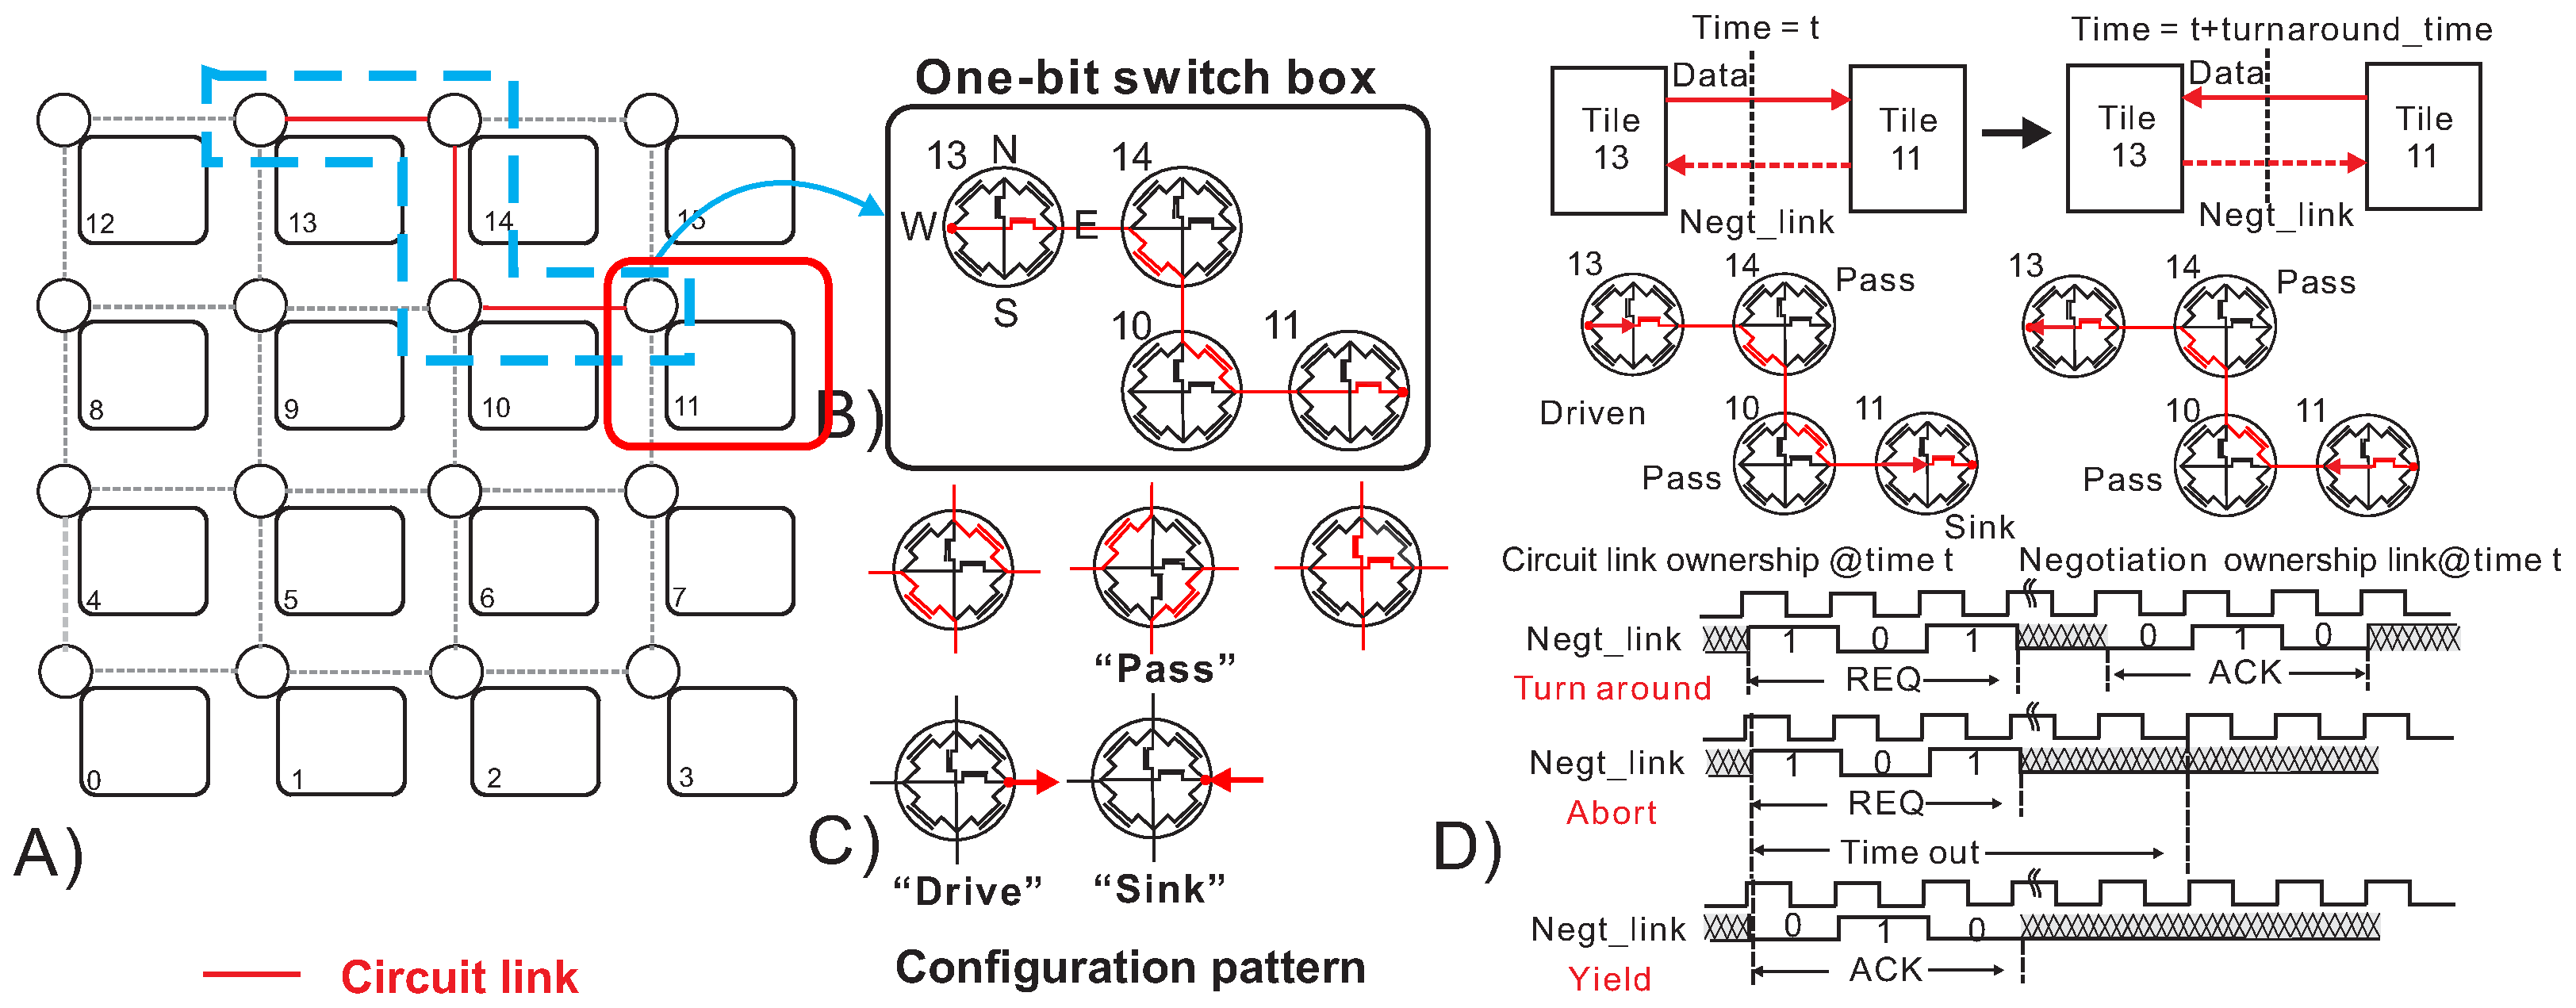
\includegraphics[width=1\columnwidth]{arch_overall.eps}
  \vskip -1mm
  \caption{\textbf{A case study: low-level architecture details} }
  \label{fig:Arch}
  \vskip -7mm
\end{figure}
\begin{algorithm}[t]
\caption{ Greedy maximization algorithm to \eqref{eq:problem_form_2}}
\label{alg:maximization}
\begin{algorithmic}[1]
\REQUIRE ~~\\
    Application  $\mathcal A(t)=(V(t),C(t);\mathcal P(\Sigma,\mathcal F))$; \\
    Reconfigurable NoC $G(t)=(N(t),E(t);\gamma(t),$$\mathcal C)$;\\
    Execution phase length $T$;
    \ENSURE ~~\\
    Compatible application partition $\pi$ and constructed circuit components set $\mathcal T$

\STATE $\pi$=Paritition$(\mathcal A(t),G(t))$
\REPEAT
\STATE $\mathcal T$=$\mathcal T \cup$ $\arg\max\limits_{T_{e}} (\mathcal G(\pi,\mathcal T \cup \mathcal T_e)- \mathcal G(\pi,\mathcal T))$
\UNTIL{$\pi$ is compatible or $\mathcal T==N(t)$}
\end{algorithmic}
\end{algorithm}
%%%%%%%%%%%%%%%%%%%%
\begin{algorithm}[t]
\caption{ $l$-relaxed Greedy maximization algorithm to \eqref{eq:problem_form_2}}
\label{alg:max_2}
\begin{algorithmic}[1]
\REQUIRE ~~\\
    Application  $\mathcal A(t)=(V(t),C(t);\mathcal P(\Sigma,\mathcal F))$; \\
    Reconfigurable NoC $G(t)=(N(t),E(t);\gamma(t),$$\mathcal C)$;\\
    Execution phase length $T$;
    \ENSURE ~~\\
    Compatible application partition $\pi$ and constructed circuit components set $\mathcal T$
\STATE $l=0$    
\STATE $\pi$=Paritition$(\mathcal A(t),G(t))$
\REPEAT
\REPEAT
\STATE $\mathcal T$=$\mathcal T \cup$ $\arg\max\limits_{T_{e}} (\mathcal G(\pi,\mathcal T \cup \mathcal T_e)- \mathcal G(\pi,\mathcal T))$
\UNTIL{$\pi$ is $l$-compatible or $\mathcal T==N(t)$ }
\IF{$\pi$ is $l$-compatible}
\STATE Return $\mathcal T$ and $\pi$
\ENDIF
\STATE $l=l+1$;
\UNTIL{$l== |\arg\max\limits_{\pi_k} |\pi_k||$}
\end{algorithmic}
\end{algorithm}

\section{Architectural Case Study}
%  \begin{figure}[htb]
%  \centering
  % Requires \usepackage{graphicx}
 % \epsfig{file=t_calc.eps}
%  \includegraphics[width=0.85\columnwidth]{negotiation.eps}
%  \caption{\textbf{Self-negotiated link driver/sink turnaround} }
%  \label{fig:negotiated}
%  \vskip -5mm
%\end{figure}
To understand how the proposed mathematical framework could be effectively applied to a reconfigurable NoC system, we consider a simple reconfigurable NoC with switch boxes to provide dedicated links, i.e., the circuit link, between different network tiles. More precisely, we study a regular mesh NoC system $G(t)=(N(t),E(t);\gamma(t))$ to which a subnet of dedicated links is attached. Formally, for each node $n_i \in N(t)$, ACF $\mathcal C$ is induced to generate a set of nodes to which a link could be set up (i.e., ACS, see Definition 5). Therefore, we have a simple reconfigurable NoC system characterized by quadruple $G(t)=(N(t),E(t);\gamma(t), \mathcal C)$. To detail the construction of ACS for each node $n_i$, we set up low-level architectural features for the switch box.

A switch box is a set of programmable pass gates. For simplicity of illustration, Figure \ref{fig:Arch}.(B) shows only the NMOS part of it. To allow circuit links to be set up between different tiles,  a switch box is organized by an array of one-bit switch boxes. The length of the array is equal to the bitwidth of a circuit link. A one-bit swap box consists of 6 pass gates such that any pair of ports can be directly connected by a dedicated link. A tile connects to a switch box through a set of similar links controlled by the pass gates. By cascading such links among a subset of nodes, it is possible to establish circuit links between them.  Figure \ref{fig:Arch}.(B) shows the configuration of a set of switch boxes such that, a set of nodes $\{n_{10},n_{11},n_{13}, n_{14}\}$ becomes a circuit component $\mathcal T_{k}$.

To simplify the hardware setup and minimize the area overhead, we assume each node in the circuit component should time-multiplex the link, i.e., one driver for any circuit link during a slotted time assigned. More precisely, for an execution time of length $T$, each node $n_{i} \in \mathcal T_{k}$ is assigned with a bandwidth, i.e., being a driver for the circuit link, proportional to its traffic share in $q(\mathcal T_{k})$.  Therefore, each switch box could work in 3 possible modes, namely, "Driver", "Sink" and "Pass" based on the ownership of the link. A switch box is in "Pass" mode if the tile connected to the switch is not the driver or sink of the data being transferred, thus "passing" the data. Otherwise, it is in "Driver" or 'Sink' mode. The working modes can be identified by the configuration pattern of switch box as shown in Figure \ref{fig:Arch}.(C). A switch box is in "Pass" mode if \textit{i}) the tile is disconnected to the switch box and \textit{ii}) switch box is programmed as any one of three configurations on top in Figure \ref{fig:Arch}.(C). Otherwise, it will be in "Driver" or "Sink".

As a simple reconfigurable NoC, we enforce the statically assigned time slot for each node in the circuit component. So there is chance that a node becomes the driver yet with no data to transmit. To maximize the link utilization in such case,  it is necessary to make possible the shift of circuit link ownership during such an idle "Driver" phase.  We thus adopt a self-negotiated link access control (SNAC) as shown in Figure \ref{fig:Arch}.(D). We build up a one-bit bi-directional negotiation link (NL) between tiles. A simple negotiation protocol is implemented over the circuit link between a driver-sink pair to bargain over the ownership. More precisely, a "Driver" during its assigned slot will automatically obtain the access to NL and the circuit link. When a data transmission is in progress, no negotiation is necessary. Otherwise, if the driver has no data to send, either a transmission is complete before the expiration of assigned time slot or no planned transmission, driver will send ACK sequence "010" to sink to yield the control over the circuit link to the sink. Upon receiving this sequence, if the sink has anything to send to the current driver, a negotiation happens: the sink will send REQ sequence "101" and wait for ACK sequence. Upon valid ACK, the sink will obtain the rest of time slot and use it for transmission to the previous driver, i.e., the sink and driver switch their roles.  Otherwise, after a preset waiting threshold, the negotiation is a failure and the sink will abort the request. In the following discussion, we will consider a set of real world applications and perform the optimization to construct circuit components by exploiting the submodularity properties of the problem as stated in~\eqref{eq:problem_form_2}.
\section{Experimental Results}
\noindent\textbf{Experiment setup:} We consider real world workloads induced by 6 SoC applications that are characterized by the proposed graphical model $\mathcal A(t)=(V(t),C(t);\mathcal P(\Sigma,\mathcal F))$. The applications include video object plan decoder (VOPD), multi-window display (MWD), MP3 encoder/decoder, H.263 encoder/decoder and MPEG-4. The number of tasks ranges from $11$ to $16$. We set up a 4x4 reconfigurable NoC described in section III as target system. The NoC system is implemented using fully synthesizable Verilog and synthesized under SMIC 65nm process using Synopsys Design Compiler with a fixed frequency constraint of 200MHz. All simulations are done using Synopsys VCS ported with Tcl scripts to load in the application traffic workloads. Throughout the simulations, NoC adopts wormhole switching for regular data transmission under variable flit-width ranging from 16-bit to 256-bit such that,  we can test the network performance under different flit injection rates given a fixed data generation rate. Each port in the router has 4 4-flit virtual channels.  We do not insert repeaters to the circuit links and assume the propagation delay should be within 1 cycle under 200MHz. Thus, we constrain the feasible size of one circuit component to be less than 5. Power estimation is done by feeding the Switching Activity Interchangeable File (SAIF) to Design Compiler during the synthesis.  We extract the switching statistics by RTL simulation in VCS and transform it into SAIF files. Algorithm \ref{alg:max_2} is implemented using C++. We use Fiduccia-Mattheyses algorithm for partition of the applications. 

\noindent\textbf{Performance evaluation:} Figure \ref{fig:task} shows the optimized network configurations for all 6 applications obtained by solving the  submodular maximization problem in (\ref{eq:problem_form_2}). Application partition $\pi$ is first obtained to minimize the cut cost, i.e., traffic between different partition components, see \eqref{eq:problem_form} for detailed explanation. Then, we run the $l$-relaxed greedy maximization algorithm to construct circuit components $\mathcal T$ such that a circuit component configuration is obtained, which is compatible with the partition $\pi$. As shown in Figure \ref{fig:task}, our algorithm identifies the critical traffic paths of all applications (see solid rectangles) and constructs circuit components (dashed rectangles) to cover most of them. An important observation is that the configuration of the network varies greatly for different applications, which suggests the spatio-temporal variability of the applications when ported to the NoC system over time. 
%We first show in Figure \ref{fig:task} the partition $\pi$ for all 6 applications and their corresponding compatible circuit components construction. To obtain feasible partitions under the physical limitations, i.e., propagation delay should be less than 1 cycle, we set the $|\pi_k| \leq 5$ for any partition component, or equivalently for any circuit component.
\begin{figure}[htb]
  \centering
  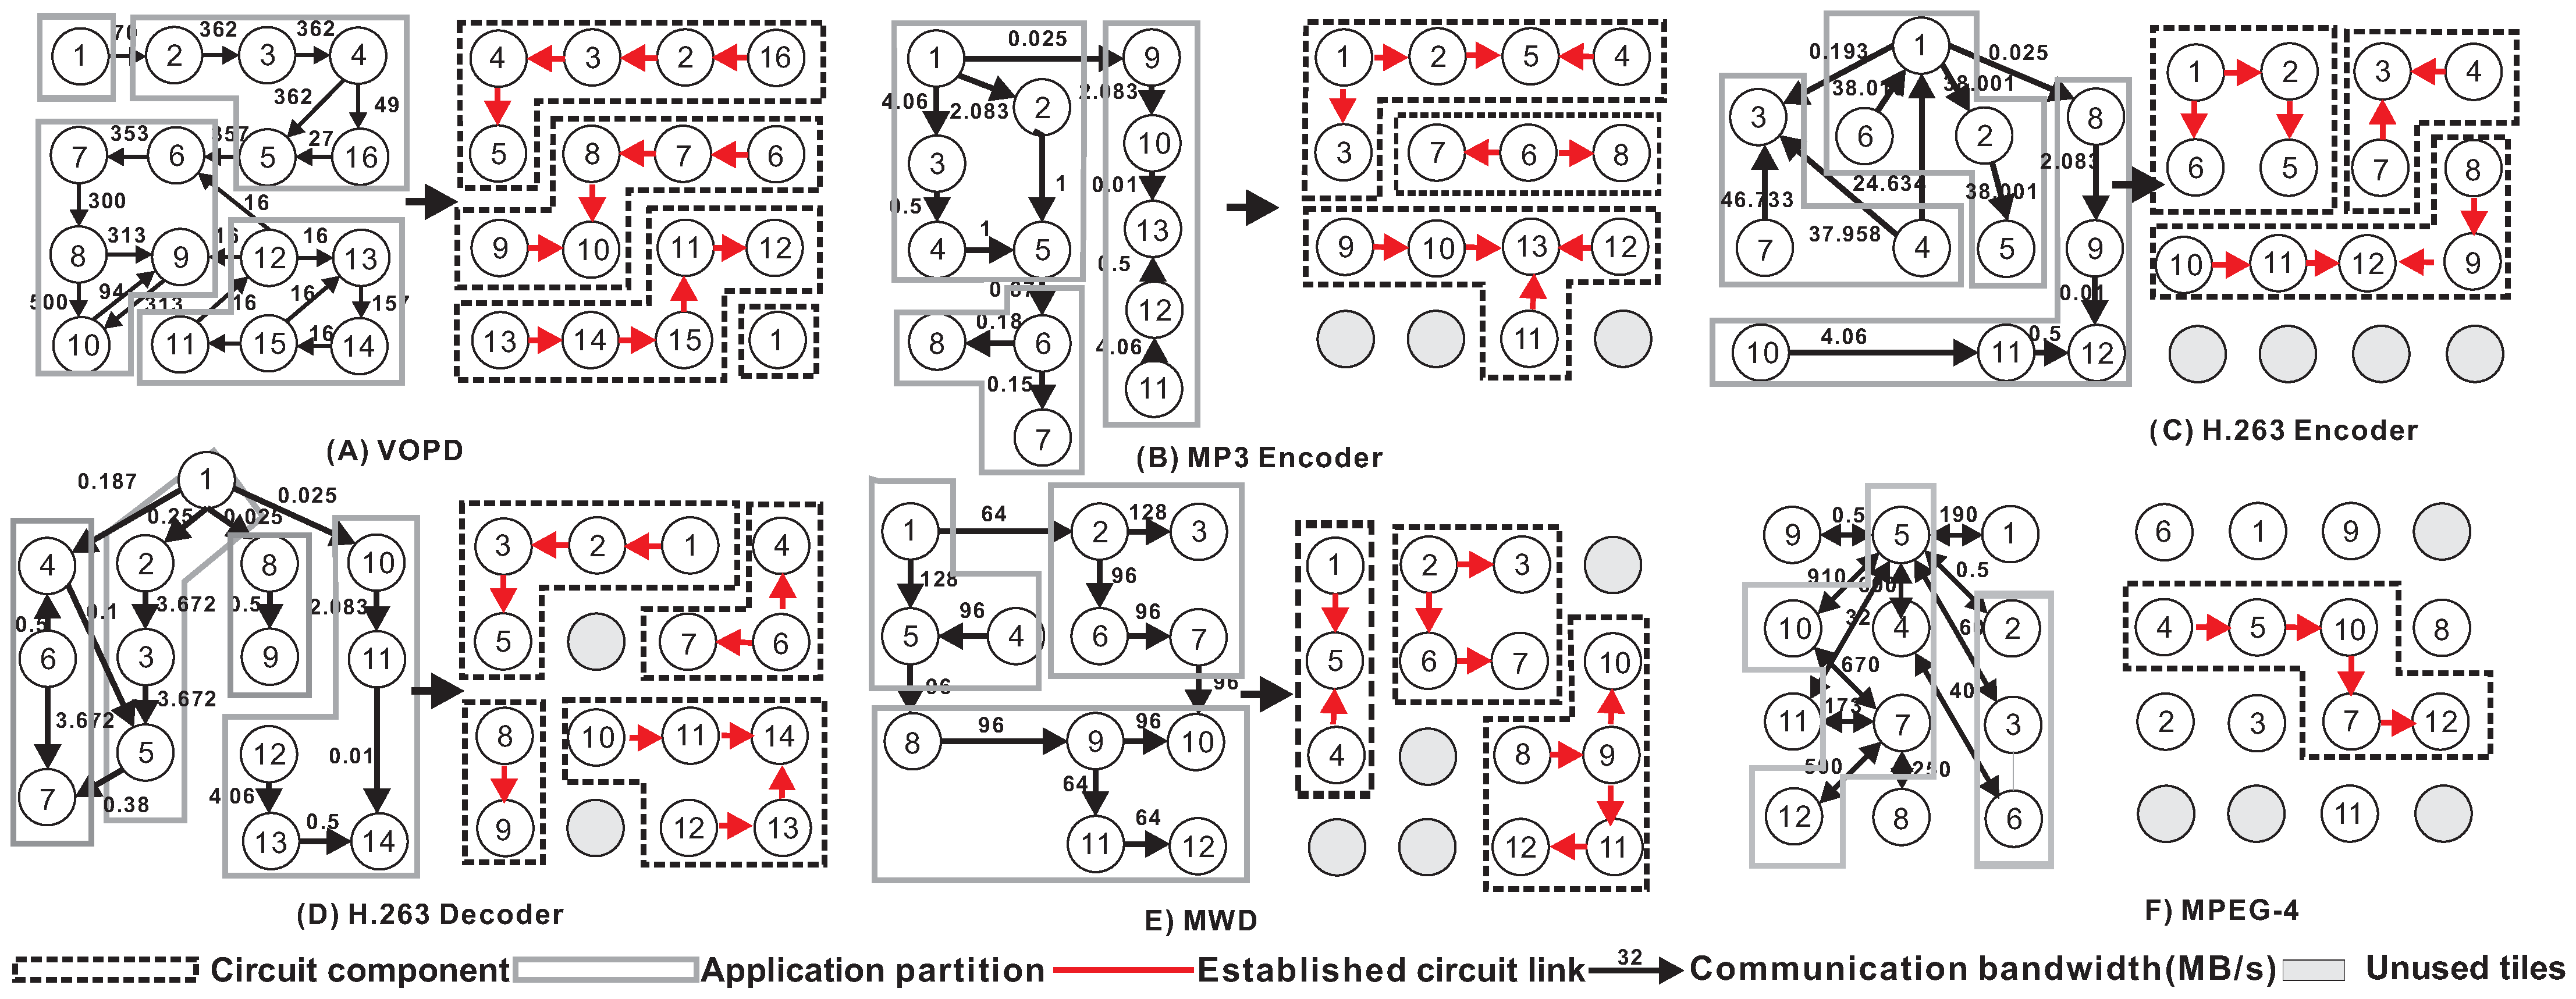
\includegraphics[width=1\columnwidth]{task_3.eps}
  \caption{\textbf{Optimized network configuration for real world applications} }
  \label{fig:task}
  \vskip -4mm
\end{figure}
\begin{figure}[htb]
  \centering
  % Requires \usepackage{graphicx}
 % \epsfig{file=t_calc.eps}
  \includegraphics[width=1\columnwidth]{main_result.eps}
  \vskip -2mm
  \caption{\textbf{Network latency and energy savings comparison between the baseline and optimized reconfigurable NoC under different traffic workloads.(a) Network latency measurements and (b) corresponding normalized energy consumptions. }}
  \label{fig:network}
  \vskip -6.5mm
\end{figure}
\indent To evaluate the performance under different traffic pressures, we run the applications on networks with different physical interconnection bandwidth (i.e., flitwidth=16-bit to 256-bit) under 200MHz to measure the network latency. In such settings, the flit injection rate has to be increased/decreased to meet the application bandwidth requirements as the physical bandwidth shrinks/grows. We compare the network latency for reconfigurable NoC optimized by Algorithm \ref{alg:max_2} and the baseline regular mesh NoC. The results are reported in Figure \ref{fig:network}.(a). For applications with smaller bandwidth requirements like MP3 Encoder, H263 Decoder and Encoder, both networks demonstrate no saturation phase transition under experimental settings. However, the optimized reconfigurable network shows on average $52.3\%$ latency reduction compared to the baseline design. This is because most of the communication with heavy traffic loads are identified and take advantage of the dedicated links without traveling through multiple routing stages.  For applications with heavy traffic requirements like VOPD, MPEG4 and MWD, the optimized network not only shows improved network latency before phase transition, but also exhibits its capability to endure greater traffic pressure, i.e., the network becomes heavily congested under a greater flit injection rate compared to the baseline design. This improvement comes from the fact that, the communication paths with heaviest traffic are covered mostly by the circuit links, thus alleviating the traffic pressure posed on the regular network.

 To show the improved energy efficiency of our optimized network, we report the normalized energy savings under different network settings in Figure \ref{fig:network}.(b). Combined with Figure \ref{fig:network}.(a), we have the following key observations: \textit{i}) Our optimized network shows improved energy efficiency ranging from $22\%$ to $38\%$ with an average of $30.2\%$, under all workloads and \textit{ii}) The energy efficiency increases as the network becomes more congested. These observations are supported by the fact that the traffic over the circuit links consumes less energy by skipping multiple routers. The energy savings are even greater when the network is congested as the recursive switching within a router for blocked packets can be avoided.
\section{Summary}
In this work, we lay the theoretical foundation for modeling the reconfigurable NoC in general and propose a mathematical framework for optimization of the NoC reconfiguration. We formulate the NoC reconfiguration as an optimization problem and prove its submodularity. Based on our theoretical analysis, we propose a greedy algorithm bounded by guaranteed optimality. As a case study, we propose a simple reconfigurable NoC as architectural instance to validate the framework. We perform the proposed optimization and evaluate it with real-world workloads. The results show a $52.3\%$ reduction of network latency on average, increased capability of handling heavy traffic and $30.2\%$ in energy reduction compared to baseline design. 
